%===============================================================================
% DOCUMENT
%===============================================================================

%% Document class
\documentclass[a4paper,12pt]{scrreprt}

%% Include packages
\usepackage{packages}

\begin{document}

%% Include custom commands
\include{commands}

\pagenumbering{gobble}

%% Build cover
\definecolor{titlepagecolor}{RGB}{37,64,56}

%==========================================================================
% COLORED BAR ON THE LEFT SIDE
%==========================================================================

\backgroundsetup{
    scale=1,
    angle=0,
    opacity=1,
    contents={
        \begin{tikzpicture}[remember picture,overlay]
            \path [fill=titlepagecolor] (-10.5,-15) rectangle ++ (5,30);
            \node[color=white] at (-6.90,-11.5) {\bfseries {\fontsize{120}{60} \textsf{C}}};
            \node[color=titlepagecolor] at (-4.30,-11.5) {\bfseries {\fontsize{120}{60} \textsf{C}}};
        \end{tikzpicture}
    }
}

%==========================================================================
% COVER PAGE CONTENT
%==========================================================================

\title{\LARGE{Network Monitoring System}}

\author{
    Flávia Alexandra da Silva Araújo (A96587)\\ \quad
    Joshua David Amaral Moreira (A105684)\\ \quad
    Miguel Torres Carvalho (A95485)\\ \quad
}

%% Date
\date{\today}

%% Course
\newcommand{\Course}{Licenciatura em Engenharia Informática}

%% Department
\newcommand{\Department}{Escola de Engenharia}

%% UniName
\newcommand{\UniName}{Universidade do Minho}

%% UniPic
\newcommand{\UniPic}{
\includegraphics[width=120pt]{img/eeum.png}}

%% University
\newcommand{\University}{
    \begin{flushleft}
        \UniPic
    \end{flushleft}
    \textcolor{gray}{\small\textbf{\textsf{\UniName}}}\par
    \textcolor{gray!80!white}{\small{\textsf{\Department}}}\par
    \textcolor{gray!70!white}{\small{\textsf{\Course}}}
}

%% UC
\newcommand{\UC}{
    \begin{flushleft}
        \par\textcolor{titlepagecolor}{\Large\textbf{\textsf{Comunicações por Computador}}}
    \end{flushleft}
}

%% Project Phase
\newcommand{\SubTitle}{
    \begin{flushleft}
        \large\textbf{Trabalho Prático 2}
    \end{flushleft}
}

%% Group Info
\newcommand{\GroupInfo}{\par Grupo 10 - PL1}

%% GitHub Repo
\newcommand{\GitHubRepo}{\par\url{https://github.com/migueltc13/CC-tp2}}

%% School Year
\newcommand{\SchoolYear}{
    \par\small{\textsf{Ano Letivo de 2024/2025}}
}

%% Define new command to show title, author and date
\makeatletter
\let\Title\@title
\let\Author\@author
\let\Date\@date
\makeatother

%==========================================================================
% BEGIN COVER PAGE
%==========================================================================

%% Make cover page
\newcommand{\makecover}{

%% Removes page number on footer
\thispagestyle{empty}

%% No indentation
\setlength{\parindent}{0em}

%% Put Background defined on \backgroundsetup, in this page
\BgThispage

%% Changing geometry to prevent overlay with text
%% At the end of back cover, geometry is default with \restoregeometry
\newgeometry{top=4cm,left=6cm,right=2cm,bottom=2cm}

%% builds university info defined previously
\University
\vspace{1cm}
\UC
\SubTitle
\SchoolYear

\vspace*{4cm}
%% bigger space (i think its the default one) between paragraphs
\setlength{\parskip}{1em}

%% builds title info defined previously
\par\textbf{\textsf{\huge\Title}}
\vspace{1cm}
%% builds author(s) info defined previously
\par\Author

\vspace{0.5cm}

%% builds date info defined previously
\par\Date
\restoregeometry
\pagebreak

}

%==========================================================================
% END COVER PAGE
%==========================================================================

\makecover

%% Default geometry
\newgeometry{top=3cm,left=3cm,right=3cm,bottom=4cm}

%% Save default geometry
\savegeometry{default}

%% Load default geometry with:
% \loadgeometry{default}

%===============================================================================
% BEGIN ABSTRACT PAGE
%===============================================================================

\renewenvironment{abstract}
 {\par\noindent\textbf{\Large\abstractname}\par\bigskip}
 {}

\begin{flushleft}
\begin{abstract}
    <<O resumo tem como objectivo descrever de forma sucinta o trabalho realizado. Deverá conter uma pequena introdução, seguida por uma breve descrição do trabalho realizado e terminando com uma indicação sumária do seu estado final.>>
    \par \textbf{Área de Aplicação}: <<Identificação da Área de trabalho.>>
    \par \textbf{Palavras-Chave}: <<Conjunto de palavras-chave que permitirão referenciar domínios de conhecimento, tecnologias, estratégias, etc., directa ou indirectamente referidos no relatório.>>
\end{abstract}
\end{flushleft}

\pagebreak

%===============================================================================
% END ABSTRACT PAGE
%===============================================================================

%===============================================================================
% BEGIN INDEXES PAGES
%===============================================================================

%% Changes table of content name
\renewcommand{\contentsname}{Índice}
\renewcommand{\listfigurename}{Índice de Figuras}
\renewcommand{\listtablename}{Índice de Tabelas}
\renewcommand{\lstlistlistingname}{Índice de \textit{Snippets}}

\tableofcontents
\pagebreak

\listoffigures
\pagebreak

\listoftables
\pagebreak

\lstlistoflistings
\pagebreak

%===============================================================================
% END INDEXES PAGES
%===============================================================================

\pagenumbering{arabic}

%===============================================================================
% BEGIN ARQUITETURA DA SOLUÇÃO
%===============================================================================

\chapter{Arquitetura da Solução}

\textcolor{red}{
    Dúvida: o diagrama da arquitetura da solução deve ser
    mais geral ou mais específico à solução (python) desenvolvida?
}

%===============================================================================
% END ARQUITETURA DA SOLUÇÃO
%===============================================================================

%===============================================================================
% BEGIN ESPECIFICACÕES DOS PROTOCOLOS APLICACIONAIS
%===============================================================================

\chapter{Especificações dos Protocolos Aplicacionais}

\section{\textit{AlertFlow}}

\subsection{Formato de Mensagem}

\subsection{Diagrama de Sequência}

\begin{itemize}
    \item Normal
\end{itemize}

\section{\textit{NetTask}}

\subsection{Formato de Mensagem}

\begin{minipage}{\textwidth}
    \centering
    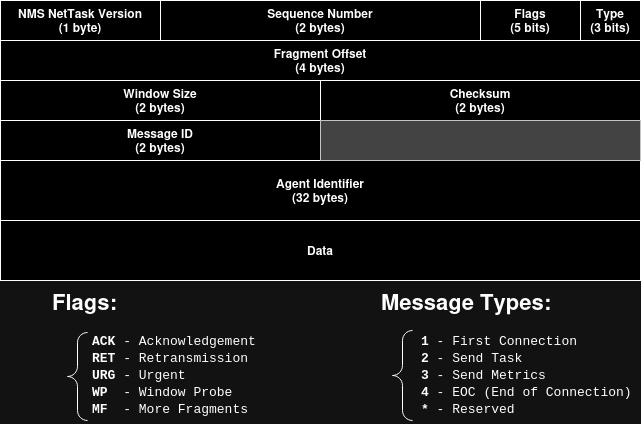
\includegraphics[width=\textwidth]{img/nettask_header.png}
    \captionof{figure}{Formato do cabeçalho do protocolo \textit{NetTask}}
    \label{fig:nettask_message_format}
\end{minipage}

\subsection{Diagramas de Sequências}

\begin{itemize}
    \item Normal
    \item Retransmission
    \item Controlo de Fluxo
\end{itemize}

%===============================================================================
% END PROTOCOLOS APLICACIONAIS
%===============================================================================

%===============================================================================
% BEGIN IMPLEMENTAÇÃO
%===============================================================================

\chapter{Implementação}

\section{\textcolor{red}{Estrutura do Projeto?}}

\section{Parâmetros dos Executáveis}

\section{Ficheiro de Configuração}

\section{Bibliotecas Utilizadas}

\textcolor{red}{
    Dúvida: deve-se referir todas as bibliotecas utilizadas no desenvolvimento? \\
    por exemplo: \textit{socket}, \textit{os}, \textit{sys}, \textit{threading}, etc
}

\section{\textcolor{red}{Detalhes Técnicos? Maybe}}

%===============================================================================
% END IMPLEMENTAÇÃO
%===============================================================================

%===============================================================================
% BEGIN TESTES E RESULTADOS
%===============================================================================

\chapter{Testes e Resultados}

\textcolor{red}{
    Para além da testagem manual contínua ao longo do desenvolvimento, foram
    desenvolvidos testes unitários para as classes e funções mais críticas do
    sistema. Estes testes foram desenvolvidos com recurso à biblioteca
    \textit{unittest} do Python.
}

%===============================================================================
% END TESTES E RESULTADOS
%===============================================================================

%===============================================================================
% BEGIN CONCLUSÕES E TRABALHO FUTURO
%===============================================================================

\chapter{Conclusões e Trabalho Futuro}

%===============================================================================
% END CONCLUSÕES E TRABALHO FUTURO
%===============================================================================

%===============================================================================
% BEGIN REFERÊNCIAS
%===============================================================================

%% Change biblibography name from “Bibliografia” to “Referências”
\renewcommand\bibname{Referências}

%% https://www.overleaf.com/learn/latex/bibliography_management_with_bibtex
\begin{thebibliography}{9}

\bibitem{DatabaseSystems}
Connolly, T., \& Begg, C. (2015). Database Systems: Example (6th ed.). Pearson Education. London, UK.

% \bibitem{MySQLManual}
% MySQL 8.0 Reference Manual (2024). \href{https://dev.mysql.com/doc/refman/8.0/en/storage-requirements.html}{MySQL 8.0 Reference Manual: Data Type Storage Requirements}. MySQL, Oracle.

\end{thebibliography}

%% Add bibliografia to index
\addcontentsline{toc}{chapter}{Bibliografia}

%===============================================================================
% END REFERÊNCIAS
%===============================================================================

%===============================================================================
% BEGIN ANEXOS
%===============================================================================

%% \addchap has no numbering but appears in table of contents.
\addchap{Anexos}

\addsec{
    \href{https://google.com/}{\small [I] Exemplo de Anexo}
    \label{anexo:1}
}

%===============================================================================
% END ANEXOS
%===============================================================================

\end{document}
